\setNextFileName{EditingJikesRVMInAnIDE.html}
\begin{section}{Editing Jikes RVM in an IDE}
\label{sec:editingjikesrvminanide}

One goal of the JikesRVM project over recent years has been the ability to develop Jikes RVM in a development environment such as Eclipse. This has been possible for the MMTk component since 2005, and as of early 2007 (release 2.9.0) it is possible to work with the majority of the Jikes RVM codebase in Eclipse and similar environments.  With Jikes RVM release 2.9.1, setting up your Eclipse environment to work with Jikes RVM became even easier.

\begin{subsection}{Editing JikesRVM in Eclipse}

These instructions assume you are working with Jikes RVM version 2.9.1 or later.

\begin{enumerate}
  \item Create a JikesRVM source tree either via Mercurial checkout or unpacking a distribution.
     \begin{lstlisting}
$ hg clone http://hg.code.sourceforge.net/p/jikesrvm/code
     \end{lstlisting}
  \item Create the machine-generated files and eclipse metadata:
     \item If you have a recent version of Jikes RVM (3.0 onwards):
       \begin{lstlisting}
$ cd jikesrvm
$ bin/buildit --eclipse localhost
       \end{lstlisting}
        \textit{Note that if you will not or cannot build on your local machine}, substitute localhost for the name of a host you can build on (buildit will perform the build remotely and then copy the requisite files back).

     \item If you are working on an older version (2.9.1 - 2.9.3), you can follow this procedure:
       \begin{lstlisting}
$ cd jikesrvm
$ ant -Dhost.name=ia32-linux -Dconfig.name=development
$ ant -Dhost.name=ia32-linux -Dconfig.name=development eclipse-project
       \end{lstlisting}
        If you will not or cannot build on your local machine:
       \begin{enumerate}
         \item copy your tree to build build host somehow
         \item perform the above ant tasks
         \item copy the following generated files and directories back to the machine you will edit on:
           \begin{itemize}
             \item jikesrvm/.project
             \item jikesrvm/.classpath
             \item jikesrvm/eclipse
           \end{itemize}
       \end{enumerate}
  \item Import the newly created Eclipse project into your Eclipse workspace.
    \begin{enumerate}
      \item From Eclipse, select File \textrightarrow\ Import
      \item Select "Existing Projects Into Workspace"
        \begin{figure}[h]
          \centering
          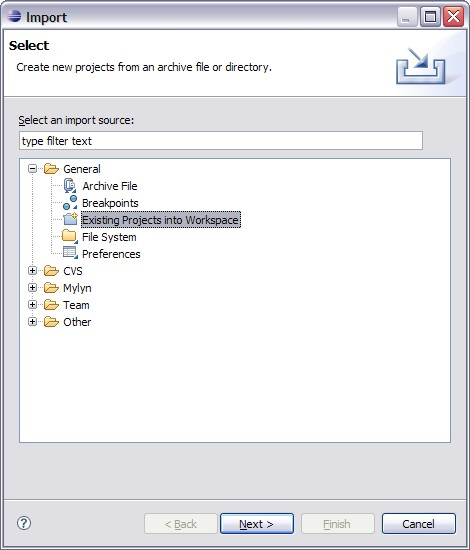
\includegraphics[width=\textwidth]{images/EditingJikesRVMInAnIDE-ImportProject.jpg}
        \end{figure}
      \item Browse to find the top-level directory.
      \item Select the project (in this case JikesRVM ia32-linux development)
        \begin{figure}[h]
          \centering
          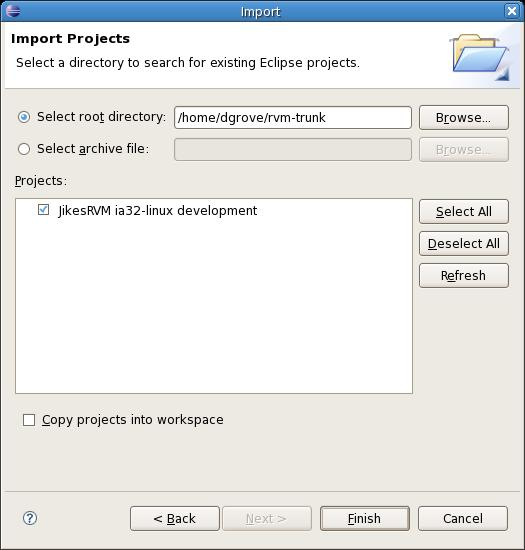
\includegraphics[width=\textwidth]{images/EditingJikesRVMInAnIDE-SelectDirectory.jpg}
        \end{figure}
      \item Hit Finish
    \end{enumerate}
\end{enumerate}

\end{subsection}

\begin{subsection}{Setup for easier compliance with the Checkstyle rules}

If you consider \href{http://www.jikesrvm.org/Contributions/}{contributing} changes back to Jikes RVM, it is helpful to configure your IDE to comply with the Jikes RVM \hyperref[sec:codingstyle]{coding style}. The coding style forbids the use of tabs and requires that no line ends with whitespace.

If you have a separate workspace for your work with Jikes RVM, you can set up Eclipse for correct tab usage by configuring the text editors. Go to Window \textrightarrow\ Preferences and then to General \textrightarrow\ Editors \textrightarrow\ Text editors (Eclipse 3.6) or Window \textrightarrow\ Preferences \textrightarrow\ General \textrightarrow\ Editors \textrightarrow\ Text Editors (Eclipse 3.5 and earlier). Check "Insert spaces for tabs". Make sure that "Displayed tab width" is set to 2. This setting affects the non-Java editors (e.g. XML editor for the ant files for the build).

To set the tab width for Java code, you need to setup the Java code style. We currently do not provide a style template, so you will have to define your own. Go to the project properties (e.g. via Project \textrightarrow\ Properties) and select Java Code Style \textrightarrow\ Formatter. Check the box "Enable project specific settings" and create a new profile for Jikes RVM. Edit the new profile. In the edit dialog, choose the tab "Indentation". Set the tab policy to "Spaces only" and set both indentation size and tab size to 2. Also make sure that the box "Empty lines" at the bottom of the "Indentation" tab is not checked.

To ensure that you do not introduce whitespace at the end of lines you can configure Eclipse's Save actions in the project properties at Java Editor \textrightarrow\ Save Actions. Check the box "Enable project specific settings" and the box "Perform the selected actions on save" as well as "Additional actions". Press "Configure" and check the box "Remove trailing whitespace" in the "Code Organizing" tab.

\end{subsection}

\begin{subsection}{Editing JikesRVM in NetBeans}

\begin{enumerate}
  \item Follow the instructions for Eclipse including building the eclipse project with ant
  \item Install the Eclipse project importer
  \item Select File \textrightarrow\ Import Project \textrightarrow\ Eclipse Project
    \begin{enumerate} 
      \item Choose to import project ignoring project dependencies
      \item Select the top-level directory you created with the JikesRVM in as the project to import
      \item Select a new folder as the destination (workspace) for the import
      \item Hit Finish
    \end{enumerate}
\end{enumerate}

\end{subsection}

\end{section}
